% %%%%%%%%%%%%%%%%%%%%%%%%%%%%%%%%%%%%%%%%%%%%%%%%%%%%%%%%%%%%%%%%%%%%%%%%%%%%%%%%%%%%%%

\subsection*{Kent Larson} 

{Director, City Science Group, Media Lab}
{Massachusetts Institute of Technology}
\subsection*{Biography}

{Kent Larson directs the City Science group at the MIT Media Lab. His research focuses on developing urban interventions that enable more entrepreneurial, livable, high-performance districts in cities. To that end, his projects include advanced simulation and augmented reality for urban design, transformable micro-housing for millennial, mobility-on-demand systems that create alternatives to private automobiles, and Urban Living Lab deployments in Hamburg, Andorra, Taipei, and Boston. Larson and researchers from his group received the “10-Year Impact Award” from UbiComp 2014. This is a “test of time” award for work that, with the benefit of hindsight, has had the greatest impact over the previous decade. Larson practiced architecture for 15 years in New York City, with design work published in Architectural Record, Progressive Architecture, Global Architecture, The New York Times, A+U, and Architectural Digest. The New York Times Review of Books selected his book, Louis I. Kahn: Unbuilt Masterworks (2000) as one of that year’s ten best books in architecture.}

%%%%%%%%%%%%%%%%%%%%%%%%%%%%%%%%%%%%%%%%%%%%%%%%%%%%%%%%%%%%%%%%%%%%%%%%%%%%%%%%%%%%%%%%%%%%%%%%%%%%%%%%%%%%%%%%%%%%%%%%%%%%%%%%%%%%%%%%%%%%%%%%%%%%%%%%%%%%%%%%%%%%%%%%%%


\subsection*{Prof. Eran Ben Joseph}

{Class of 1922 Professor of Landscape Architecture and Urban Planning, head of the Department of Urban Studies and Planning at MIT from 2013 to 2020}
% 
\subsection*{Biography}
{Eran Ben-Joseph is the Class of 1922 Professor of Landscape Architecture and Urban Planning in the Department of Urban Studies and Planning at the Massachusetts Institute of Technology. Eran served as Head of the Department of Urban Studies and Planning at MIT from 2013 to 2020. His research and teaching areas include urban and physical design, standards and regulations, sustainable site planning technologies and urban retrofitting. He authored and co-authored the books: Streets and the Shaping of Towns and Cities, Regulating Place: Standards and the Shaping of Urban America, The Code of the City, RENEW Town and ReThinking a Lot. Eran worked as a city planner, urban designer and landscape architect in Europe, Asia, the Middle East and the United States on projects including new towns and residential developments, streetscapes, stream restorations, and parks and recreation planning. He has led national and international multi-disciplinary projects in Singapore, Barcelona, Santiago, Tokyo and Washington DC among other places. Eran holds degrees from the University of California at Berkeley and Chiba National University of Japan. Current Research: Urban Form and Health, Urban Form and the Aging Population, Urban Form and Ecological Models of Development, Urban Form and Manufacturing.}

%%%%%%%%%%%%%%%%%%%%%%%%%%%%%%%%%%%%%%%%%%%%%%%%%%%%%%%%%%%%%%%%%%%%%%%%%%%%%%%%%%%%%%%%%%%%%%%%%%%%%%%%%%%%%%%%%%%%%%%%%%%%%%%%%%%%%%%%%%%%%%%%%%%%%%%%%%%%%%%%%%%%%%%%%%


\subsection*{Prof. Esteban Moro}

{Associate professor at the Universidad Carlos III de Madrid (Spain). Visiting Professor, Media Lab, Massachusetts Institute of Technology}
% 
\subsection*{Biography}
% 
{Prof. Esteban Moro is a visiting professor at the MIT Media Lab, an associate professor at the Universidad Carlos III de Madrid (Spain) and a member of the Joint Institute UC3M-Santander on Financial Big Data. Prof. Moro serve as a consultant for many public and private institutions and have held previous positions at the University of Oxford, Institute of Knowledge Engineering (Spain), and Instituto Mixto de Ciencias Matemáticas (Spain).Moro research is on applied mathematics, financial mathematics, viral marketing, and social networks. He received the "Shared University Award" from IBM in 2007 for modeling the spread of information in social networks and application to viral marketing and the Research Excellence Awards in 2013 and 2015 from the Carlos III University of Madrid. His recent work has been covered by many media outlets, including articles and interviews in El Pais, Muy Interesante, The Atlantic, The Washington Post, and The Wall Street Journal.}

% \newpage

%%%%%%%%%%%%%%%%%%%%%%%%%%%%%%%%%%%%%%%%%%%%%%%%%%%%%%%%%%%%%%%%%%%%%%%%%%%%%%%%%%%%%%%%%%%%%%%%%%%%%%%%%%%%%%%%

\section{Introduction}
\subsection{Problem Statement}

{The massive move to densely populated areas during the 20th century has a bipolar effect on cities and their planning mechanisms: On the one hand, urbanization brings clear economic benefits, reduction of poverty, agglomeration of knowledge and innovation, improved public health, and sustainable energy consumption \cite{Glaeser2011, reckien2017climate, banerjee2011companion}. On the other hand, massive urban migration, entangled with climate change, technological disruptions, and inequality, can become unsustainable for traditional urban mechanisms \cite{parnell2016defining, reckien2017climate}. With over 50\% of the world population living today in urban areas, and projected two-thirds by 2050, city-planning practitioners face unprecedented planning challenges \cite{united2018world, UnitedNationsHabitatIII2017}.} 

{Amidst these growing challenges, legacy planning and decision-making processes are rendered insufficient \cite{Ben-Joseph2004, green2019smart, gaffney2018smarter}. Slow moving planning processes lag behind population growth; monolithic regulations struggle with technological disruptions; scarcity of data and evidence-based processes stifle urban decision-making \cite{world2016inspiring, grauman1976orders, chen2014global}. These issues can also encourage development patterns that neglect proper scrutiny, `cut corners', and fail to provide the basic needs of well-preforming cities \cite{banerjee2011companion}. Under these circumstances, urban decision-makers are forced to reactivally respond rather than pre-plan.}

{During the past two decades, the tech industry recognized these challenges, and sought to replace legacy urban processes with rapid, scalable, data driven and evidence based solutions \cite{soderstrom2014smart}. Under the title of `Smart Cities', these efforts sought to optimize urban environments using strategies, technologies and methods imported from the Silicon-Valley. Yet after over a decade of real-world experiments, most `Smart Cities' use-cases failed to offer comprehensive solutions and instead were materialized through sporadic optimizations to legacy systems. \cite{green2019smart, gaffney2018smarter}. Even if successful in some domain, these solutions often overlook the complexity of cities and the ever-changing needs of their inhabitants \cite{gaffney2018smarter}. In addition, many Smart Cities solutions surfaced new concerns in the context of technology and cities, such as bias, inequality, privacy, and misuse \cite{green2019smart}.} 

{In this respect, an ever-growing urban world is now facing a planning dilemma: both traditional urban processes, as well as new `smart' solutions cannot efficiently respond to the emerging challenges of 21st century cities \cite{soderstrom2014smart}.}

 

 %%%%%%%%%%%%%%%%%%%%%%%%%%%%%%%%%%%%%%%%%%%%%%%%%%%%%%%%%%%%%%%%%%%%%%%%%%%%%%
\subsection{Proposed Contribution}

{In this dissertation I propose an alternative human-centric, urban planning and decision-making process. I examine this emerging process through the design, development and real-world deployment of \textbf{CityScope}: an urban modeling, simulation and decision-making platform, that meets urban technology with social discourse. CityScope proposes a set of comprehensive, community-driven, adaptable, and iterative technologies, that confront planning questions from the point of view of citizens \cite{batty2013new, habitat2016new}. In the UN-Habitat III (2016), the need for a new human-centric, planning technology was recognized and manifested at the `New Urban Agenda': {\textit{``The New Urban Agenda presents a paradigm shift based on the science of cities; it lays out standards and principles for the planning, construction, development, management, and improvement of urban areas (...) We will foster the creation (...) of open, user-friendly and participatory data platforms using technological and social tools available to transfer and share knowledge (...) to enhance effective urban planning and management.''}} \cite{habitat2016new}.This thesis extends on four major themes of CityScope development and deployments: (i) insight, (ii) prediction, (iii) transformation, and (vi) consensus:}

{\textbf{Insight and Prediction:} New spatial analytics and urban-modeling techniques, novel data resources as well as new processing methodologies, can augment participatory planning with real-time insights and predictions \cite{salganik_bit_2017, Kitchin2014, Ben-Joseph2001}. Data-driven methods (such as Machine-Learning and Deep-Learning models) can expedite the investigation of complex planning scenarios and their effects on human dynamics, traffic, energy-use, or economic performance \cite{Foth2011, Song2010}. This dissertation explores new ways to collect, analyze, model, and communicate urban insights and predictions.} 

{\textbf{Transformations:} Urban-design, scenario testing, and spatial intervention through iterative exploration. Interactive technologies, including Virtual, Augmented, and Mixed Reality, Computer-Vision, web-based applications and even robotics can support iterative participation processes. These technologies allow users to explore, dynamically change and create numerous planning scenarios side-by-side, in both physical and virtual environments. Design iterations could simultaneously be evaluated for their trade-offs and Key Performance Indicators (KPIs), in an ``apples-to-apples'' comparison \cite{Ishii2002}. This kind of synchronous design process does not only lower cost and expedite the search for solutions, but can also expose unpredictable designs.}


 %%%%%%%%%%%%%%%%%%%%%%%%%%%%%%%%%%%%%%%%%%%%%%%%%%%%%%%%%%%%%%%%%%%%%%%%%%%%%%

\begin{figure}[t]
\begin{center}
   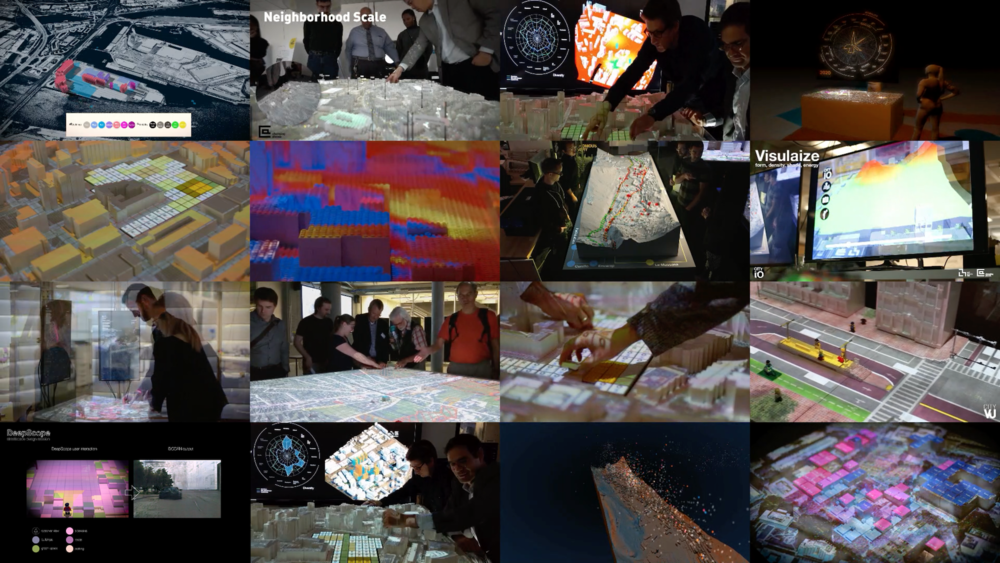
\includegraphics[width=0.9\linewidth]{figures/all_projects.png}
\end{center}
   \caption{CityScope projects and deployments(from top left): Grasbrook, BRT neighborhood scale, Volpe, Paris, Volpe, Observatory, Andorra, CityScopeAR, MoCho, FindingPlaces, Volpe, BRT street scale, DeepScope, Volpe, Reversed Urbanism, MoCho}
\label{fig:all_projects}
\end{figure}
 
 %%%%%%%%%%%%%%%%%%%%%%%%%%%%%%%%%%%%%%%%%%%%%%%%%%%%%%%%%%%%%%%%%%%%%%%%%%%%%%

{\textbf{Consensus and Collaborative Governance:} Constructing consensus-driven decision-making processes. The ability to engage multiple stakeholders simultaneously is a fundamental aspect in a new urban process \cite{Ben-Joseph2004}. Unlike traditional systems, these tools are designed around large-scale, shared public spaces (physical or virtual) that can facilitate multiple participants and conversations at once. This can reduce the bureaucratic overhead of negotiating in different channels, thus prompting concise, result-driven participation sessions \cite{Ben-Joseph2001, Innes2016}.}



{This thesis contributes to urban modeling and simulation, HCI systems, and Decision Support Systems in several aspects:
\begin{itemize}
    \setlength\itemsep{0em}
	\item The development of a scalable, real-time, socio-technical urban modelling and simulation platform.
	\item A system for distributed urban analytics through decentralized computation system. 
	\item The development of novel analytics modules to asses urban behavior, mobility, and performance. 
	\item Deployment of numerous CityScope platforms around the world, several in real-world city-planning contexts.
	\item The creation of community of users, developers, contributes, and researchers building and using CityScope worldwide.  
\end{itemize}
}
\newpage
%%%%%%%%%%%%%%%%%%%%%%%%%%%%%%%%%%%%%%%%%%%%%%%%%%%%%%%%%%%%%%%%%%%%%%%%%%%%%%%%%%%%%%%%%%%%%%%%%%%%%%%%%%%%%%%%
\newpage
\subsection{Publications, Projects, and Deployments Summary}
\subsubsection{Publications}

This dissertation will build on my recent work which has appeared in conferences and journals as listed below:

{\textbf{Noyman, A.}, Larson, K. (2020, April). DeepScope: HCI Platform for Generative Cityscape Visualization. In Extended Abstracts of the 2020 CHI Conference on Human Factors in Computing Systems (pp. 1-9).}

{\textbf{Noyman, A.}, Doorley, R., Xiong, Z., Alonso, L., Grignard, A., Larson, K. (2019). Reversed urbanism: Inferring urban performance through behavioral patterns in temporal telecom data. Environment and Planning B: Urban Analytics and City Science, 46(8), 1480-1498.}

{Doorley, R., \textbf{Noyman, A.}, Sakai, Y., Larson, K. (2019). What’s your MoCho? Real-time Mode Choice Prediction Using Discrete Choice Models and a HCI Platform.}

{Alonso, L., Zhang, Y. R., Grignard, \textbf{A., Noyman}, A., Sakai, Y., ElKatsha, M., Larson, K. (2018, July). Cityscope: a data-driven interactive simulation tool for urban design. Use case volpe. In International conference on complex systems (pp. 253-261). Springer, Cham.}

{\textbf{Noyman, Ariel}, Yasushi Sakai, and Kent Larson. "Cityscope{AR}: urban design and crowdsourced engagement platform." arXiv preprint arXiv:1907.08586 (2019).}

{Grignard, A., Macià, N., Alonso Pastor, L.,\textbf{Noyman, A.}, Zhang, Y., Larson, K. (2018, July). Cityscope andorra: A multi-level interactive and tangible agent-based visualization. In Proceedings of the 17th International Conference on Autonomous Agents and MultiAgent Systems (pp. 1939-1940).
}
{\textbf{Noyman, A.}, Holtz, T., Kröger, J., Noennig, J. R., Larson, K. (2017). Finding places: HCI platform for public participation in refugees’ accommodation process. Procedia computer science, 112, 2463-2472.}

{Alrashed, T., Almalki, A., Aldawood, T., \textbf{Noyman, A.}, ... Alwabil, A. (2015). An observational study of usability in collaborative tangible interfaces for complex planning systems. Procedia Manufacturing, 3, 1974-1980.}

{\textbf{Noyman, A.} (2015). POWER/STRUCTURES: the Urban Form of Regulations (SM Thesis, Massachusetts Institute of Technology).}
% 
\begin{sidewaystable}
\subsubsection{CityScope Development and Deployments}
{This dissertation will build and extend CityScope projects developed at MIT, and deployed in real-world use-cases:}
\\\\
% \begin{table}[ht]
\centering
\begin{adjustbox}{width=\textwidth}
\begin{tabular}{llllll}
\textit{project} & \textit{description} & \textit{medium}  &\textit{deployment} &\textit{date}  &  \\ \hline
CityScope Kendall Square & Urban Data Observatory & TUI & MIT Media Lab & 2013-2016 &  \\
CityScope Playground & Zoning simulator & TUI & APA, Cambridge City Council & 2014-2015&\\
CityScope BRT & Dudley Square & TUI, SW & Boston & 2014-2015\\
CityScope FindingPlaces & refugees’ accommodation process & TUI & Hamburg, Germany & 2015-2016\\
CityScopeAR & Augmented and Mixed Reality system for CityScope & AR/MR SW & Andorra, Volpe, BRT, APA & 2016-2019\\
CityScope Andorra & Telecom data observatory & TUI & Smart Cities Summit, Barcelona & 2016\\
CityScope Andorra & Urban Simulation and decision-making & TUI & Andorra La Vella & 2016-2017\\
CityScpoe LivingLine & Evaluating commercial street performance & TUI & Shanghai, China &  2017-2020\\
Reversed Urbanism & Human behavioral patterns through discrete telecom data & WEB & MIT Media Lab & 2018\\
CityScpoe MoCho & Modelling Mobility Mode Choice & WEB & MIT Media Lab & 2019\\
DeepScope & Predicting urban streetscapes through Generative models & TUI & MIT Media Lab & 2019\\
CityScope Champs-Élysées & Predicting interventions impact for Champs Élysées & TUI & Paris & 2019-2020\\
CityScope Corktown & Simulating real-time planning and mobility scenarios &  SW WEB & Ford, Detroit & 2019-2020\\

\hline
\textit{Work In Progress}\\
\hline
CityScope Volpe & City Simulation & TUI & MIT Media Lab & 2016-\\
CityScope Grasbrook & System for evaluating design competition proposals & TUI &  MIT and Hamburg & 2018-\\

CityIO & CityScope distributed backend & SW  &  MIT,  CSLs & 2016-\\

RoboScope & Robotic Interface for CityScope & TUI & Media Lab & 2019-\\

CityScopeJS & CityScope Distributed Web Platform
 & WEB & Across City Science Network & 2018-\\

\end{tabular}
\end{adjustbox}

\begin{minipage}{0.6\textwidth}
    \fontsize{8}{6}\selectfont
    \begin{enumerate}[topsep=1pt,itemsep=-1.5ex,partopsep=0.5ex,parsep=1ex]
        \item CSjs GRACIO
        \item CSjs Detroit Ford-Land
        \item CSjs Jerusalem
        \item CSjs Ho Chi Minh City District 4
        \item CSjs East Palo Alto
        \item CSjs `21 City Science Network course 
    \end{enumerate}
\end{minipage}


\end{sidewaystable}


\newpage


\subsubsection{CityScope Milestones}
{This list include milestones of the CityScope project, including exhibitions, awards, and mentions in popular media.}


\begin{itemize}

\item{CityScope was featured in “Report to The President - Technology and the Future of Cities”, President’s Council of Advisors on Science and Technology, 2016 (pp. 23)}

\item{CityScope project presented in the ‘Road Ahead’ exhibition at the Cooper Hewitt, NY 2019.}

\item{“FindingPlaces”: Public participation process using CityScope for data-driven housing allocation and planning for 80,000 refugees} 
    
\item{OECD Observatory for Public Sector Innovation (OPSI) and the United Arab Emirates (UAE) Mohammed Bin Rashid Centre for Government Innovation (MBRCGI) selected “FindingPlaces” out of 600 submission as a `Global Innovation': https://trends2019.oecd-opsi.org/}
    
\item{“FindingPlaces” won the United Nations - “Urban Act Award”, https://urbact.eu/finding-places}

\item{Poon, L. (2015, October 16). MIT's New Interactive LEGO Urban Tool Brings Transparency to Transit Planning. Retrieved July 26, 2020, from https://www.bloomberg.com/news/articles/2015-10-16/mit-s-new-interactive-lego-urban-tool-brings-transparency-to-transit-planning}

\item{Gillies, C. (2014, December 18). Lego: Can this most analogue of toys really be a modern urban planning tool? Retrieved July 26, 2020, from https://www.theguardian.com/cities/2014/dec/18/lego-toys-urban-planning-tool-architects-mit}

\item{Making ideas into reality at MIT's "Future Factory". (n.d.). Retrieved July 26, 2020, from https://www.cbsnews.com/news/60-minutes-mit-media-lab-making-ideas-into-reality-future-factory-2019-08-04/}
\item{Rob Matheson | MIT News Office. (2017, October 13). Small European nation becomes a "living lab" for urban innovation researchers. Retrieved July 26, 2020, from http://news.mit.edu/2017/european-nation-andorra-living-lab-media-lab-urban-innovation-1013}

\item{Science of Teams: Science of Teams. (2017, January 23). Science of Teams: How MIT Media Lab Builds Cities Using Lego and Augmented Reality. Retrieved July 26, 2020, from https://www.wired.com/video/watch/science-of-teams-mit-media-lab}

\item{Prevost, L. (2018, April 03). Building a Connected City From the Ground Up. Retrieved July 26, 2020, from https://www.nytimes.com/2018/04/03/business/smart-city.html}

\item{Wener-Fligner, Z. (2014, December 19). Lego makes a monochrome set targeted at architects. Retrieved July 26, 2020, from https://qz.com/315776/lego-for-grown-ups-the-toy-maker-is-targeting-architects-and-urban-planners/}

\item{GOLDSMITH, BOUSQUET, AR is Transforming Tech. What Can It Do for Cities?. Retrieved July 26, 2020, from https://datasmart.ash.harvard.edu/news/article/ar-transforming-tech-what-can-it-do-cities}

\item{LAURA ADLER,. (2016, AUGUST 29). SimCities: Can City Planning Mistakes Be Avoided Through Data-Driven Simulations? Retrieved July 26, 2020, from https://www.govtech.com/data/SimCities-Can-City-Planning-Mistakes-Be-Avoided-Through-Data-Driven-Simulations.html}

\item{Garcia, J. (2018, July 08). El MIT usa fichas Lego y big data para saber dónde dar futuro a los inmigrantes. Retrieved July 26, 2020, from https://www.lainformacion.com/tecnologia/el-mit-salva-inmigrantes-con-fichas-lego-gracias-al-big-data-sabe-donde-deben-ser-situados-en-una-ciudad/6351916/}

\item{Woldin, P. (2016, March 02). „City-Scope": Mit Legosteinen Flüchtlingsunterkünfte finden - WELT. Retrieved July 26, 2020, from https://www.welt.de/regionales/hamburg/article152836431/Mit-Legosteinen-Fluechtlingsunterkuenfte-finden.html}

\end{itemize}

\newpage
\newpage
%%%%%%%%%%%%%%%%%%%%%%%%%%%%%%%%%%%%%%%%%%%%%%%%%%%%%%%%%%%%%%%%%%%%%%%%%%%%%%%%%%%%%%%%%%%%%%%%%%%%%%%%%%%%%%%%%%%%%%%%%%%%%%%%%%%%%%%%%%%%%%%%%%%%%%%%%%%%%%%%%%%%%%%%%%
\section{Background and Related Work}

{Since the turn of the century, unprecedented urbanization, technological disruptions, and economic turmoil increased the pressure on traditional city-planning mechanisms \cite{parnell2016defining, UnitedNationsHabitatIII2017}. To mitigate housing and infrastructure shortages, cities worldwide are forced to abandon slow-moving planning processes in favor of hyper-localized interventions \cite{banerjee2011companion}. These ad-hoc solutions often resulted with low-tier urban expansions, which lack proper physical and social infrastructure \cite{Glaeser2011, MARCHETTI199475}.}

{Despite advancements in spatial analytics and the abundance of data, contemporary urban decision - making processes are still heavily fragmented and inconsistent \cite{branch1978critical, banerjee2011companion, Ben-Joseph2004}. The literature observes various factors contributing to the insufficiency of legacy planning processes: Contemporary urban research still lacks necessary scientific background, does not accompanied by evidence-based decision-making, and is ill-prepared to interact with rapid changes in policy \cite{banerjee2011companion, McPhearson2016}. Even when cities attempt to modernized their decision-making processes,they still need to confront the scarcity and inaccessibility to data, and cannot effectively assess changes as they occurs \cite{bulmer_how_2001}.}

{To address some of these challenges, data-drive and collaborative urban decision-making platforms emerged already in the 1960's \cite{Ben-Joseph2001, Ishii2002, banerjee2011companion}. Yet few of these experiments proposed iterative, and collaborative urban decision-making systems, that can provide high-end and real-time spatial analytics \cite{Snyder2003, mueller2018citizen}. Even fewer systems matured to take part in real-world planing and decision-making processes. This section explores the origins, and attempts to create alternative planning systems and processes. It discusses past, current, and future research on urban HCI principles, platforms, and processes.}

\subsection{Collaborative Urban Process}

{The legal framework empowering citizens participation in city-planning dates back to the 1950's \cite{banerjee2011companion}. Despite decades of participatory planning, many attempts to incorporate citizens in urban decision-making were criticised for their lack of transparency, politicization, and privatization \cite{Innes2016}. As Arenstien argues, the regulatory enforcement of institutionalized participation paradoxically reduced the ``citizen power'' to mere tokenism \cite{arnstein1969ladder}. In recent years, a demand for a new decision making model emerged by both practitioners as well as knowledgeable citizens \cite{green2019smart, Glaeser2011, gaffney2018smarter}. This new model was manifested by the UN's `New Urban Agenda': \textit{``We will foster the creation (...) of open, user-friendly and participatory data platforms using technological and social tools available to transfer and share knowledge."} \cite{habitat2016new}}

{Such `paradigm shift' demands a comprehensive, community-driven, and iterative urban process, which places technology in the service of diverse stakeholders \cite{soderstrom2014smart}. This alternative process can create what Hou describers `citizen experts', armed with access to information, planning and design knowledge, acting as proactive public participants \cite{banerjee2011companion}. The usage of new tools that are inherently open for interpretation and critical review can also promote `Collaborative Participation'. As Innes proposes, joint fact finding should be conducted by parties who can use participation to question the data, models and insights \cite{Innes2016}.}

\subsection{Urban HCI}

{The emergence of advanced socio-technical systems, as well as new techniques for urban modeling and simulation, created the opportunity to meet the NUA goal for \textit{"open, user-friendly and participatory data platforms"}. These methodologies embrace the ubiquity of connected devices, `big-data', and high-end processing power to create a new socio-technical forum for discussion and decision-making \cite{batty2013new, Ben-Joseph2001}.}

\begin{figure}[t]
\begin{center}
    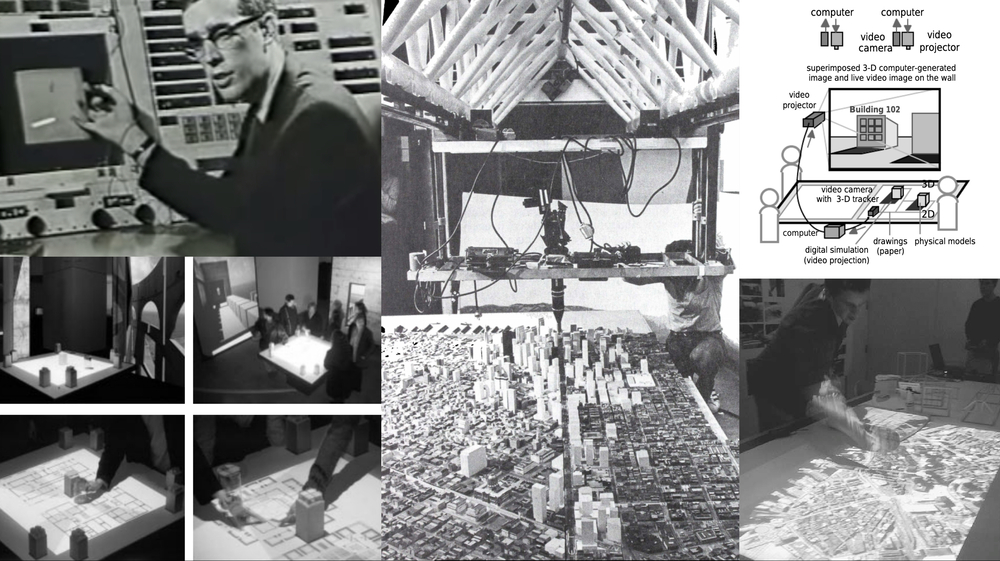
\includegraphics[width=0.9\textwidth]{figures/urbanHCI.jpg}
\end{center}
   \caption{Urban HCI milestones. Spanning over five decades, these systems aspired to combine the agility and rapidness of computational systems, with the ease of use and collaborative manner of tangible interfaces.    
   (top left) Sutherland, "Sketchpad" (1963),
   (bottom left)  Larson, "Louis I. Kahn: Unbuilt Masterworks" (1999),
   (center) Bosselmann, "The Berkeley Environmental Simulation Laboratory (1984),
   (right) Ben-Joseph, "luminous planning table" (2001)
   }
\label{fig:urbanHCI}
\end{figure}

{Since the 1960's, urban HCU researchers embraced the idea of collaborative and shared design environments, engaging professionals and non-professionals alike in the planning discourse \cite{Ben-Joseph2004, Ishii2008}. Although different in their design, purpose, and usage pattern, these tools share similar themes: (I) their design supports collaborative decision-making; (II) they promote playful and iterative design and feedback-loops; (III) and they are expected to respond in a near real-time manner \cite{Ullmer2010, Ben-Joseph2001, Snyder2003, mueller2018citizen}.}


\textbf{Multi-Stakeholders:}{A key component of urban HCI is the ability to engage multiple stakeholders at once \cite{Ben-Joseph2004}. Unlike traditional design and CAD interfaces, these platforms are built around large-scale, shared public spaces (physical or virtual) that can facilitate many participants. This can reduce the bureaucratic overhead of negotiating in different channels, and promote concise, result-driven participation sessions \cite{Ben-Joseph2001}. In the last few decades, urban HCI platforms were developed to facilitate collaborative urban design, augmented by computational analytics. Notably are the Environmental Simulation Laboratory (ESL) in Berkeley \cite{bosselmann1984berkeley}, URP \cite{underkoffler1999urp}, and the Augmented Urban Planning Workbench \cite{Ben-Joseph2004}, all built for collaboration in various stages of the urban process.}

{With the rise of internet, efforts to extend collaboration and participation beyond the limits of physical spaces brought these technologies to the virtual sphere. Using connected devices and shared virtual `sandboxes', planning discussions could also occur remotely, thus extending the number of potential participants in an order of magnitude \cite{Ben-Joseph2013, banerjee2011companion, green2019smart}. Advancements in Virtual, Augmented, and Mixed Reality, could allow remote participants to immersively understand, discuss, and reach consensus \cite{bulmer_how_2001}.}

\textbf{Iterative Urban Design:}{ }{Modern HCI technologies, including Virtual, Augmented, and Mixed Reality, Computer-Vision, advanced web applications, rapid-prototyping, and robotics can support iterative participation processes. Prior art include the I/O Bulb, The Clay Table and Sensetable \cite{Ishii2004, Ishii2002, Ishii2008} which converged the digital and the physical in seamless design-feedback loops. These systems allowed side-by-side comparison in both physical and virtual environments, in which each design iteration was only a starting point for an another design. Unlike linear design processes, this approach created a graph of potential design iterations with minimal overhead and virtually no cost. Different designs could then be evaluated for their trade-offs and Key Performance Indicators (KPIs), in an ``apples-to-apples'' comparison \cite{Ishii2002}. This kind of synchronous design process does not only expedite the designers work, but can also expose edge-cases and `out of the box' design solutions.}

\textbf{Interactive, Real-time Analytics:}
{Modern spatial analytics and urban-modeling techniques can serve urban HCI platforms with real-time data and high-end insights \cite{Kitchin2014, salganik_bit_2017}. Emerging modeling techniques, such as Machine-Learning and Deep-Learning, can expedite the investigation of complex planning scenarios and their effects on human dynamics, traffic, energy-use, or economic performance. Although some of these modelling techniques are not new, they were traditionally limited to experts, and their complexity required significant time and resources, making them less fit for real-time applications \cite{Foth2011}.}

\subsection {The Limits of a New Urban Process}

{Urban HCI platforms can transcend lengthy, inefficient, and costly planning processes. Current breakthroughs in Data Science could augment these systems with real-time urban analytics \cite{Barbosa-Filho2017}. Affordable computation and immersion technology can help better communicate design alternatives, their impacts and KPIs. Nevertheless, with the emergence of new technologies, new challenges arise, and several traditional issues still remain. This dissertation will address two aspects of urban HCI challenges: (I) technical limitations, such as accessibility, accuracy of models and data, and possible bias, as well as (II) the perils of `techno-utopia' and overreliance on technology. }



\newpage
%%%%%%%%%%%%%%%%%%%%%%%%%%%%%%%%%%%%%%%%%%%%%%%%%%%%%%%%%%%%%%%%%%%%%%%%%%%%%%%%%%%%%%%%%%%%%%%%%%%%%%%%%%%%%%%%%%%%%%%%%%%%%%%%%%%%%%%%%%%%%%%%%%%%%%%%%%%%%%%%%%%%%%%%%%
\section{Research Plan}

{This dissertation proposes an alternative model for urban-decision making. This model embodies a systematic, scalable, evidence-based and data-driven approach, alongside a comprehensive, long-term, and community driven planning. This \textit{New Urban Process}, is manifested in the design, development and deployment of CityScope. CityScope is a human-centered, urban modeling, simulation and decision-making platform, that merges urban technology with social discourse. This section reports on a series of lab experiments and real-world deployments of the CityScope platform, as well as on-going and future CityScope projects.}


\begin{figure}[t]
\begin{center}
    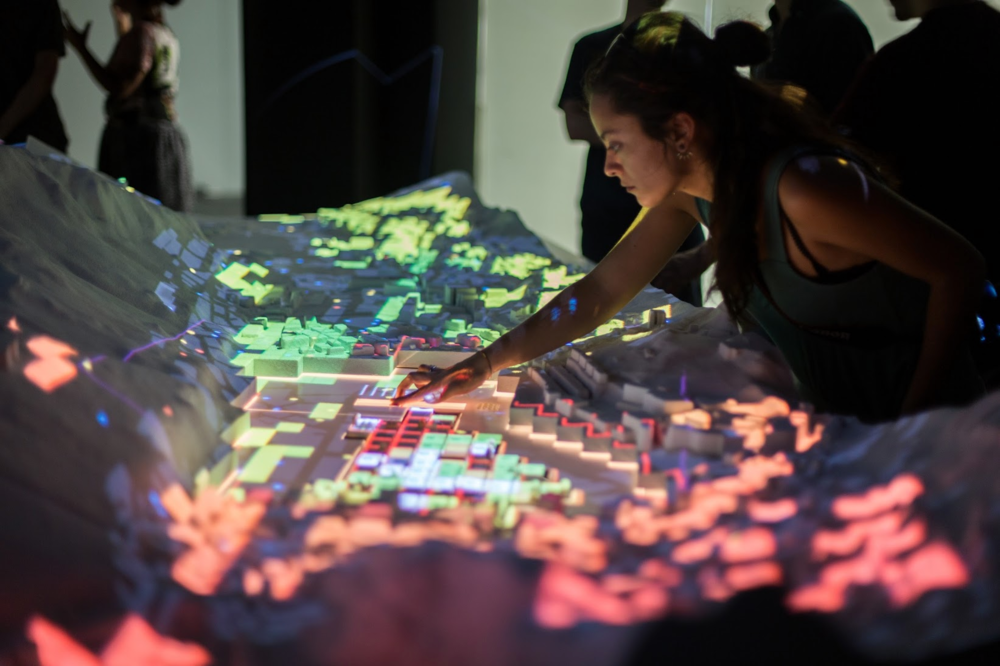
\includegraphics[width=\textwidth]{figures/csl_andorra.png}
\end{center}
   \caption{CityScope Andorra at the City Science Lab in Caldea, Andorra la Vella. Built in 2016, this platform was one of the first to serve as an interactive, real-time tool for urban decision making in real world settings. Here, a user interacts with a Tangible User Interface to asses the impacts of different interventions in the city center.}
\label{fig:csl_andorra}
\end{figure}


\subsection{CityScope: Development Themes}

{Since 2013, CityScope is being developed at the MIT City Science Group, as well as by research labs, companies, and individuals around the world. In this section I cluster CityScope milestones into four major categories: \textbf{Insight}: CityScope as urban observatory, expending on advanced methods in urban and spatial analysis, and focusing on high-resolution, geolocated, urban-dynamics data. \textbf{Predictions}: turning insights into forecasts, using methods of urban modelling and simulation, with an emphasis on real-time predictive models. \textbf{Transformations}: building iterative spatial 'what-if' scenarios through playful and exploratory process. Developing multiple urban-HCI methodologies to engage diverse parties in the urban process. \textbf{Consensus}: Using CityScope to construct multi-stakeholder decision-making, consensus and policy recommendations. Explores Socio-technical systems to facilitate collaborative and distributed urban decision-making.}



\begin{figure}
\begin{center}
    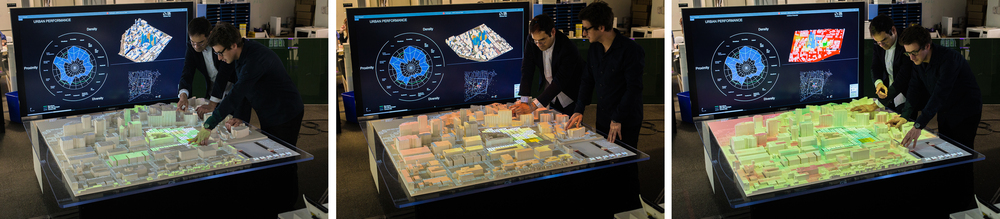
\includegraphics[width=\textwidth]{figures/volpe_all.jpg}
\end{center}
   \caption{CityScope Volpe. This interface explores the development efforts around the MIT campus - DOT Volpe facility. As users interact with the TUI, different matrices update in real-time, to augment multi-party decision-making process. }
\label{fig:volpe_all}
\end{figure}

%%%%%%%%%%%%%%%%%%%%%%%%%%%%%%%%%%%%%%%%%%% 
%%%%%%%%%%%%%%%%%%%%%%%%%%%%%%%%%%%%%%%%%%% 
%%%%%%%%%%%%%%%%%%%%%%%%%%%%%%%%%%%%%%%%%%% 

\subsection{Insight: Observing the City's Current State}

{Urban insights help understand the current state of the city, and can highlight areas in need for change. As highly complex systems of systems \cite{Batty2009}, it is often challenging to focus the planning process on the right urban questions. Narrowing the spectrum of urban observations is a step towards a productive discourse between stakeholders and decision makers. Methodical data collection and representation can also set the stage for more accurate scenarios testing. Early CityScope instances focused on augmenting accessible and concise urban data onto physical 3D platforms, in an effort to facilitate conversations on the city's current performance and plausible interventions. The \textbf{Urban Data Observatory} (2013-2016), displayed various pre-computed urban insights of the MIT and Kendall Square area, such as urban form, physical systems, solar emission, or wind regime.}

{In later CityScope projects, early data exploration and visualization is used to inform the research question and establish KPIs for urban interventions. In \textbf{CityScope Andorra} (2016), observations from Call Data Records and Radio Network Controller data were used to interpret discrete mobility trajectories. Insights gathered from this data could suggest how people move, by which modes of transportation, their daily routines, congregation spots, and the points of interest that attract them. These insights helped create interactive CityScope platforms that can support urban-planning, traffic and energy optimisation, tourism management, as well as COVID-19 mobility policies.}

\begin{figure}
\begin{center}
    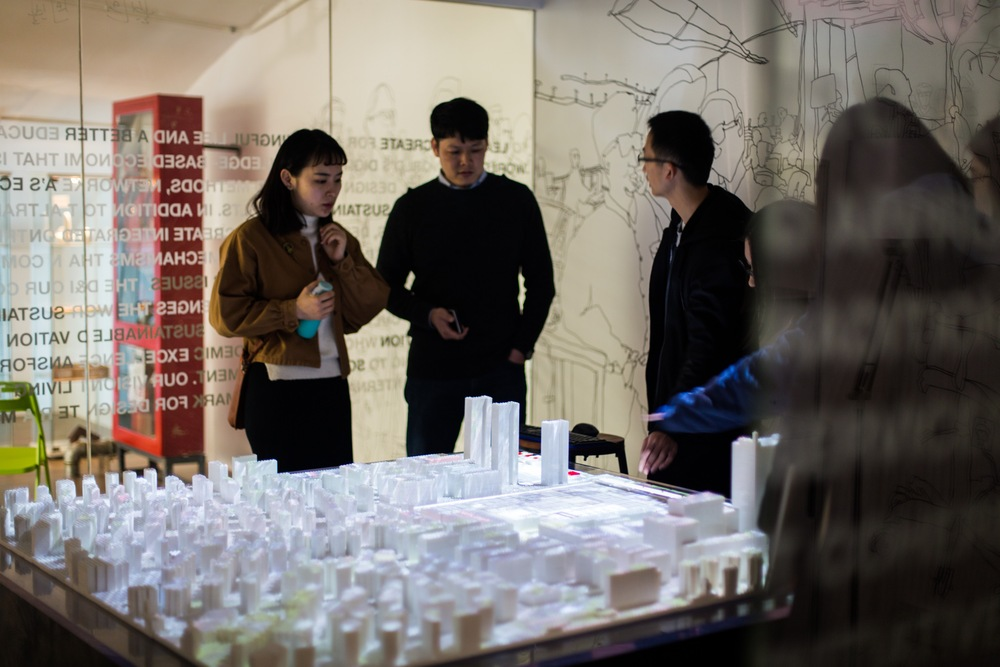
\includegraphics[width=\textwidth]{figures/CSL_tongji.jpg}
\end{center}
   \caption{CityScope LivingLine in Tongji University, Shanghai. Insights with no data: The lack of spatial and behavioral data in this site was compensated by hands-on data aggregation conducted by troves of students.}
\label{fig:CSL_tongji}
\end{figure}

{In places where Location Base Service data is scarce or unavailable, more traditional approach to street observation and data collection can be used. In \textbf{CityScope LivingLine} (2017) in Shanghai, street surveys and physical counts were performed to evaluate small-scale human mobility within a busy shopping area. Similar methodology was  used for the CityScope project in \textbf{Aalto University Campus} in Espoo, Helsinki (2017), where large group of students gathered usage patterns of the campus facilities. Although these methods of data collection are limited, fine-grained recollections of human behavior can go beyond the static representation of spaces, functions and urban systems, and shed light on discrete aspects of urban performance.}

{This thesis will include results from several \textit{insight} related projects, including: Hi-res clustering and analysis of streets vibrancy in Boston; and investigation into the relationship between mobility and COVID-19 spread in Andorra}


\subsection{Transformation}

{The role of CityScope's insights is to focus the discussion on specific urban challenges, and establish clear KPIs to evaluate future interventions. The third step in \textit{a new urban process} is transformation, in which iterative exploration of interventions and policies is performed. In CityScope, testing transformation alternatives is possible through a slew of urban-HCI methodologies and interfaces. Unlike traditional planning and design practices, CityScope is built for dynamic scenario exploration, in which evaluation is conducted synchronously. To allow for fast iterations and real-time feedback, transformation capability is developed via two parallel streams: (i) The creation of iterative user interfaces, such as Tangible User Interfaces, AR, VR, MR, and web-based UIs. (ii) real-time models, simulations, and KPI results which can provide feedback during design sessions.}

\begin{figure}[t]
\begin{center}
    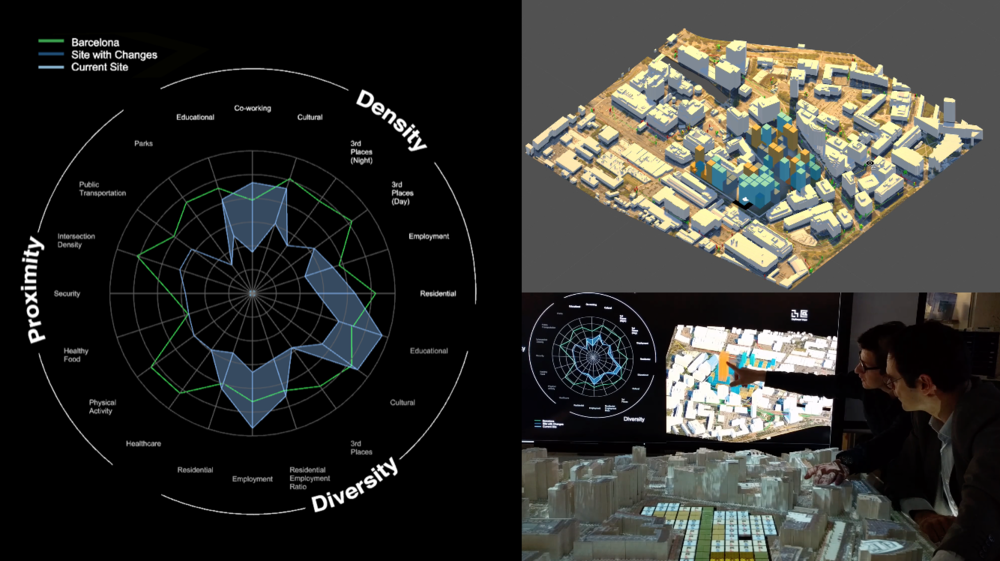
\includegraphics[width=0.8\textwidth]{figures/volpe_ui.png}
\end{center}
   \caption{Urban transformation. Left: a set of KPIs and urban indicators are evaluated with each design iteration. Upper-right: The users interactions are translated to three-dimensional zoning envelops, which represent the maximal intervention framework, rather than actual building volumes. Lower-right: Users are presented with both outputs as a mean to direct their design collaboration process.}
\label{fig:volpe_ui}
\end{figure}


{Different HCI methods were developed in order to digitally capture virtual and physical objects and translate users' interaction into urban transformation. In \textbf{CityScope Playground} (2014-2015), and in the vast majority of CityScope TUIs, a scanning of tagged LEGO bricks allowed near real-time physical-digital interaction. \textbf{CityScopeAR} (2015-2017) added Augmented, Mixed, and Virtual Reality environments that extend CityScope tangible interface. Deployed in the context of \textbf{Boston BRT}, \textbf{Andorra}, and \textbf{Volpe} CityScope projects, this system allowed to enlarge the user-base of participants and curate specific insights to each user. A unified system for obtaining user-interaction from AR devices, LEGO and robotic TUI, and web interfaces was introduced in \textbf{CityScopeJS} (2019).}


{\textit{Transformation} is also the phase in which real-world constraints, such as spatial and legal boundaries are introduced. In \textbf{CityScope Playground}, (2014-2015) an urban simulator design to evaluate building-code and zoning, users explored how existing zoning laws might impact future developments, and suggest zoning amendments. Later transformation projects, such as \textbf{Volpe} (2016-2017), \textbf{Andorra}, (Andorra La Vella 2016-2017), \textbf{Grasbrook} (Hamburg, 2018), and \textbf{Corktown} (Detroit, 2020) included additional site analyses, such as accessibility, spatial diversity of land-use and functions, and various mobility aspects.}

{This thesis will include results from several \textit{transformation} projects, including: the development of a web-based, platform agnostic interaction system for Cityscope; The development of a data standard across CityScope projects; the integration of different TUIs into the platform, such CV based system, actuated interface, as well as touch and web UI.}

%%%%%%%%%%%%%%%%%%%%%%%%%%%%%%%%%%%%%%%%%%% 
%%%%%%%%%%%%%%%%%%%%%%%%%%%%%%%%%%%%%%%%%%% 
%%%%%%%%%%%%%%%%%%%%%%%%%%%%%%%%%%%%%%%%%%% 

\subsection{Prediction: Urban `What-if' Scenarios}

{The ability to predict the future of urban environments is a critical aspect in urban planning, urban design, and architecture. Unlike other industries, urban interventions rarely permit processes of trial-and-error and A/B testing, thus requiring high degree of confidence and well established predictive models \cite{doi:10.1080/14649357.2015.1127994}. As depicted in figure \ref{fig:axis}, urban predictions could be generally described using two vectors: (I) the prediction time-frame, and (II) the social to physical spectrum.}

\begin{figure}[t]
\begin{center}
    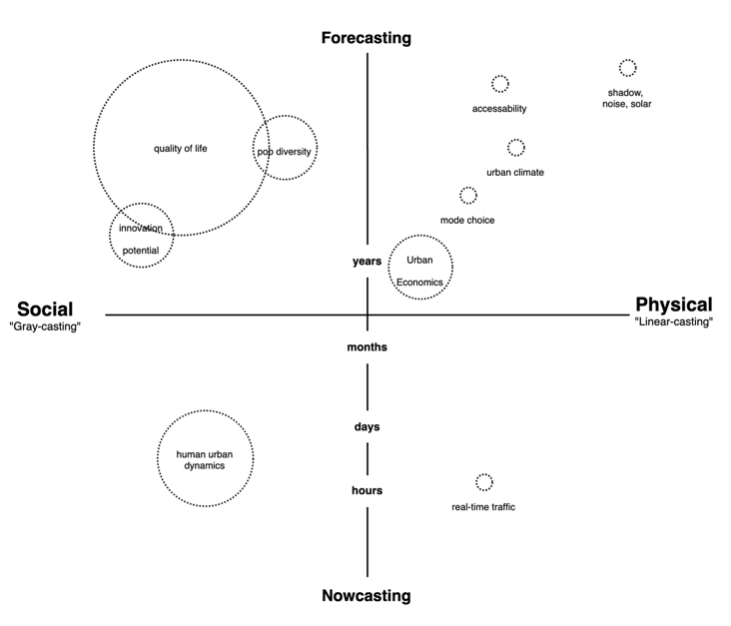
\includegraphics[width=0.7\textwidth]{figures/prediction_axes.png}
\end{center}
   \caption{The landscape of urban prediction. The horizontal axis represents the degree of `concreteness' of each prediction (social <-> physical). The vertical axis depicts the longevity of the prediction (now <-> far future).}
\label{fig:axis}
\end{figure}

{As an example, predicting the shadow effect of a new building on the streetscape is linearly correlated to its bulk and shape. Evidently, as long as the world spins around the sun, the results of shadow modelling should be consistent, and the model describing this phenomena could be reused indefinitely. On the other end, a predictive model of potential human interaction in a public plaza, would share much less consistency across time and space. This model would heavily rely on social and cultural aspects, as well as physical attributes of the urban realm (such as the plaza's shape, or its proximity to certain amenities). This class of predictions, which focuses on human-urban dynamics, is dramatically harder to construct, validate and reuse, but can carry greater impact on decision-making.}

{Today, many commercial and research tools already offer high-accuracy and efficiency in physical urban prediction. This dissertation focuses on the other class of predictions, at the intersection of human behavior and the built environment. The \textbf{Reversed Urbanism} (2017-2018) project attempted to model and predict the propensity of certain human behavioral patterns in public spaces
 (see figure \ref{fig:revurb}). These models meshed geo-spatial attributes (such as urban form, POIs, and street network graphs), and socio-behavioral properties, interpreted from high-resolution telecom data. Later CityScope projects, such \textbf{Corktown}, and \textbf{Grasbrook} take similar approach when meshing geospatial data with hi-res location data to conduct mobility predictions.}



\begin{figure}[t]
\begin{center}
    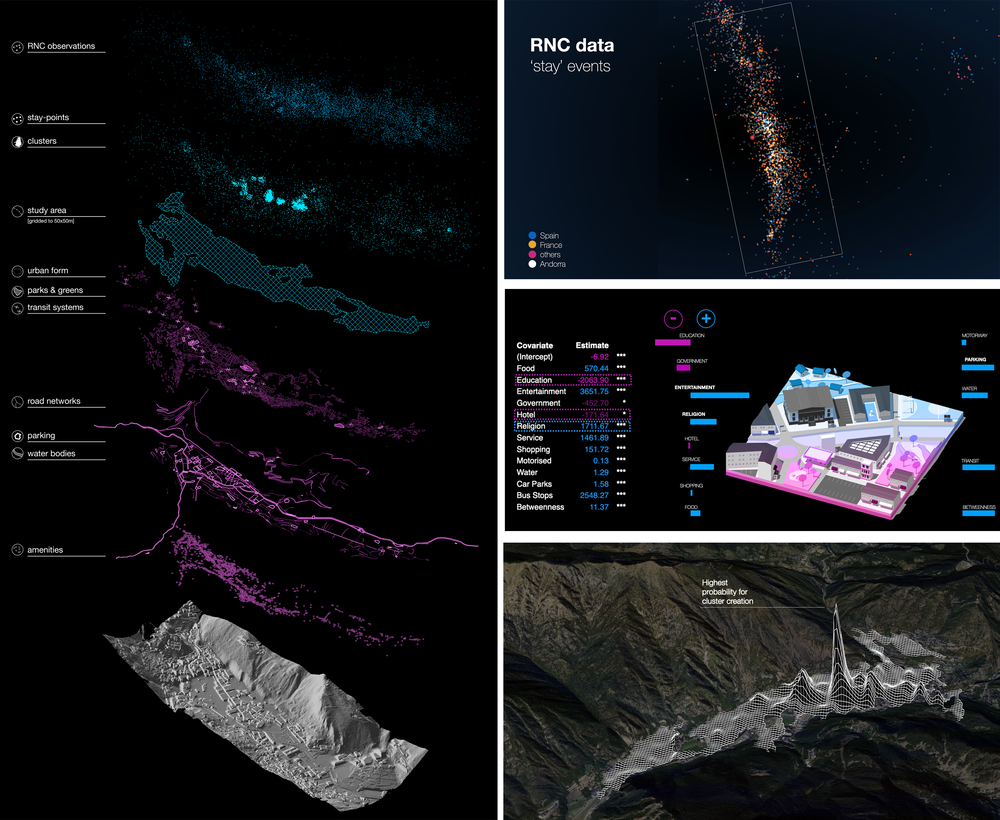
\includegraphics[width=0.9\textwidth]{figures/revurb.png}
\end{center}
   \caption{The Reversed Urbanism project. Left: various layers of spatial and behavioral data are meshed to create a spatio-temporal understanding of the cityscape. Upper-right: high-resolution geo-located telecom data is processed as `stay events', in which users stayed above a certain spatio-temporal threshold. Mid-right: The degree of correlation between clusters of stay-events and different spatial features are modelled for each cell on an arbitrary grid. Lower-right: the model can then predict the propensity of each cell to attract these clustered behaviors.}
   
\label{fig:revurb}
\end{figure}

{When geo-located data are scarce or unavailable, other techniques could be used to simulate urban dynamics. In \textbf{CityScope MoCho} (2019), mobility mode-choice patterns for the Boston metro area were simulated using synthetic population. Static data, such as census and National Household Travel Survey (NHTS) were used to construct simulated profiles of daily commuters. By interpreting plausible trips from socio-demographic data, the model could predict how fairly small scale changes to land-use (performed via CityScope TUI) can affect large scale mobility behaviors.}

{Simulated populations can also help to understand emergence and agglomeration patterns, and can inform design decisions. In CityScope \textbf{Volpe}, \textbf{Andorra}, \textbf{Grasbrook} and \textbf{Champs-Élysées} (2016-2020) Agent Based Models (ABM) are used to simulate travel patterns and mobility choices as a result of land-use and urban-design transformations. A similar approach was used in the \textbf{Hamburg Port-City Model}, in which an ABM was used to predicate changes to tourist activity in train-stations and the harbor port. In these cases, when mobility data was insufficient, virtual populations were formed to model and predict the impact of urban intervention. }


\begin{figure}[t]
\begin{center}
    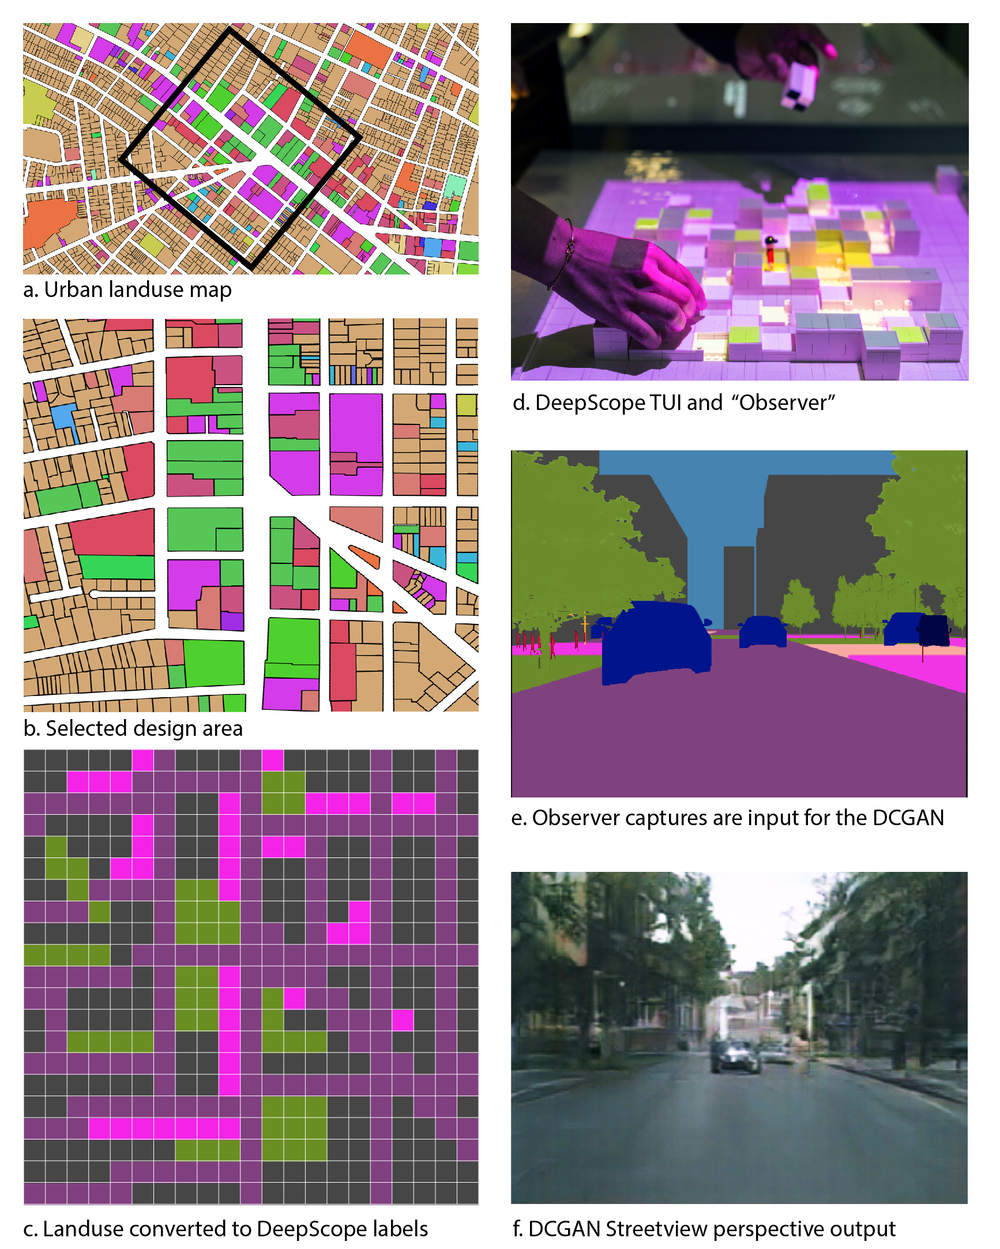
\includegraphics[width=0.6\textwidth]{figures/landuse.jpg}
\end{center}
   \caption{DeepScope module: (a,b) designating an urban intervention site (c) translating the site's land-use/zoning bounds and (d) user-interaction into (e) procedural 3D environment and (e) passing it to DCGAN model for generation of a street-view visualization}
\label{fig:landuse}
\end{figure}
{A different aspect of CityScope predictions involves the usage of data-driven models to forecast changes in urban environments. These models can expedite traditionally complex and slow urban analytics, as well as generate a slew of possible iterations for each design question. The \textbf{DeepScope} (2019) project uses Generative Adversarial Networks to predict and render streetscapes of areas under development in real-time. The goal of this CityScope module is to expedite traditional urban design processes, and offer real-time visualization during early massing exercises. Similar models use Convolutional Neural Networks to expedite CityScope predictive capabilities (such as innovation potential, urban mobility, economic performance, sustainable buildings, or community benefits), and replace them with pre-trained, real-time predictions.}

{This thesis will include results from several \textit{prediction} projects, including: the development and testing of real-time modelling framework for CityScope; publication of real-time mobility model for Detroit; and the usage of pre-trained machine learning models to reduce computation overhead in Hamburg.}

\begin{figure}[t]
\begin{center}
    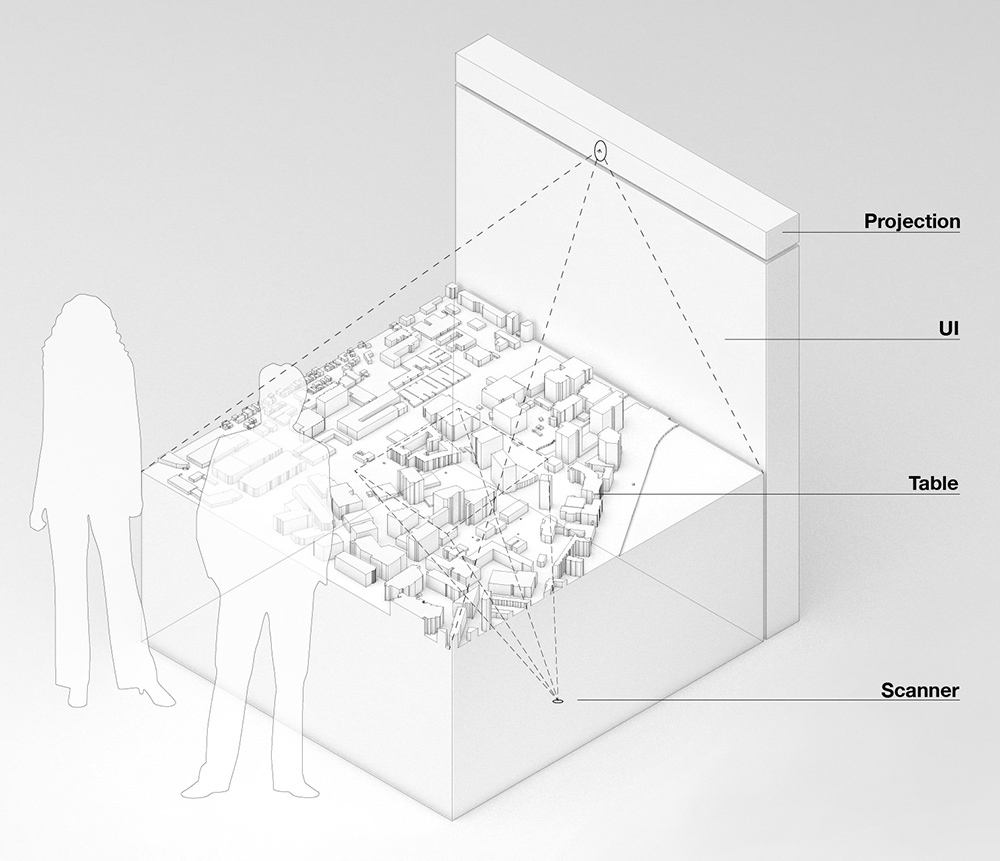
\includegraphics[width=0.6\textwidth]{figures/CityScope TUI.jpg}
\end{center}
   \caption{Common architecture of CityScope TUI: Multiple users can simultaneously interact and discuss urban design iterations. The table-top is used as both the design space and a schematic urban top-view. The vertical monitor visualizes additional insights and predictions. Sensors/cameras scan the scene for real-time interaction.}
\label{fig:CityScopeTUI}
\end{figure}

%%%%%%%%%%%%%%%%%%%%%%%%%%%%%%%%%%%%%%%%%%% 
%%%%%%%%%%%%%%%%%%%%%%%%%%%%%%%%%%%%%%%%%%% 
%%%%%%%%%%%%%%%%%%%%%%%%%%%%%%%%%%%%%%%%%%% 

\subsection{Consensus}

{The last phase, and probably the most impactful in \textit{the New Urban Process} is the establishment of consensus between diverse stakeholders. Too often, planning processes are invested in the envisioning of urban futures through data, simulation, and design iterations, but fail to include stakeholders and the public in these processes.} 

{In the core of CityScope is the notion that planning efforts must be conducted in a shared, collaborative, and engaged way. This approach promoted the design of the platform, the development of its computational models and modules, as well as the creation of community engagement processes that revolve around these technologies. \textbf{CityScope Boston BRT} (2014-2015), a community engagement process for the planning on Bus Rapid Transit routes, brought together a range of urban HCI technologies with public participation. This process aimed to go beyond common community engagement sessions which range between information-sharing to venting, and instead was designed around co-creation and citizen-driven planning. In this case, CityScope was not only a planning and urban transformation tool, but also as a medium supporting debate and evidence-based discourse by different parties.}


\begin{figure}[!tbp]
  \centering
  \begin{minipage}[b]{0.48\textwidth}
    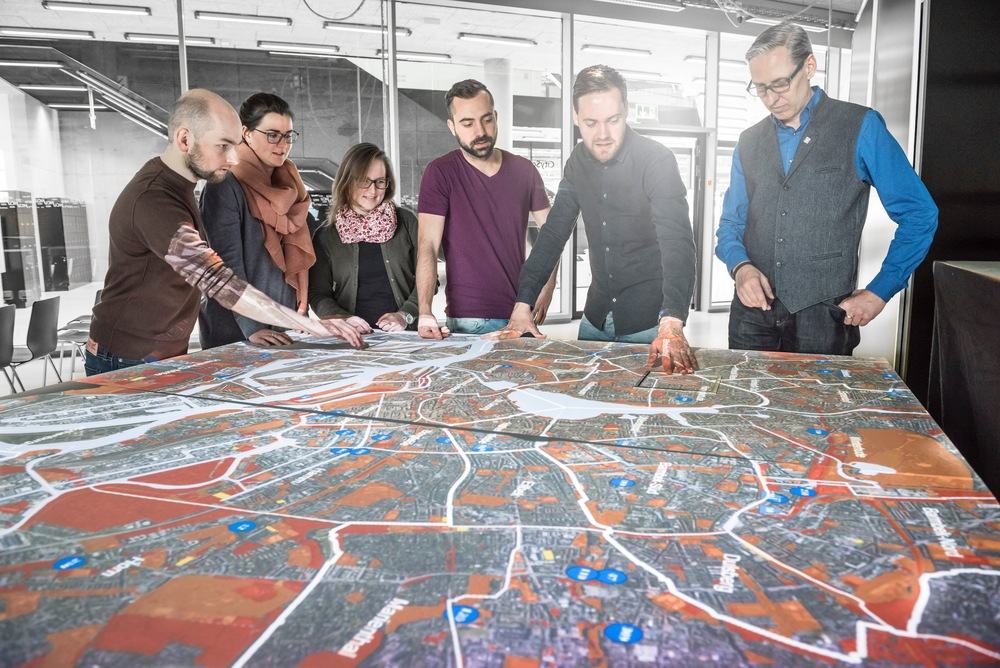
\includegraphics[width=\textwidth]{figures/finidingplaces1.jpg}
  \end{minipage}
  \hfill
  \begin{minipage}[b]{0.48\textwidth}
   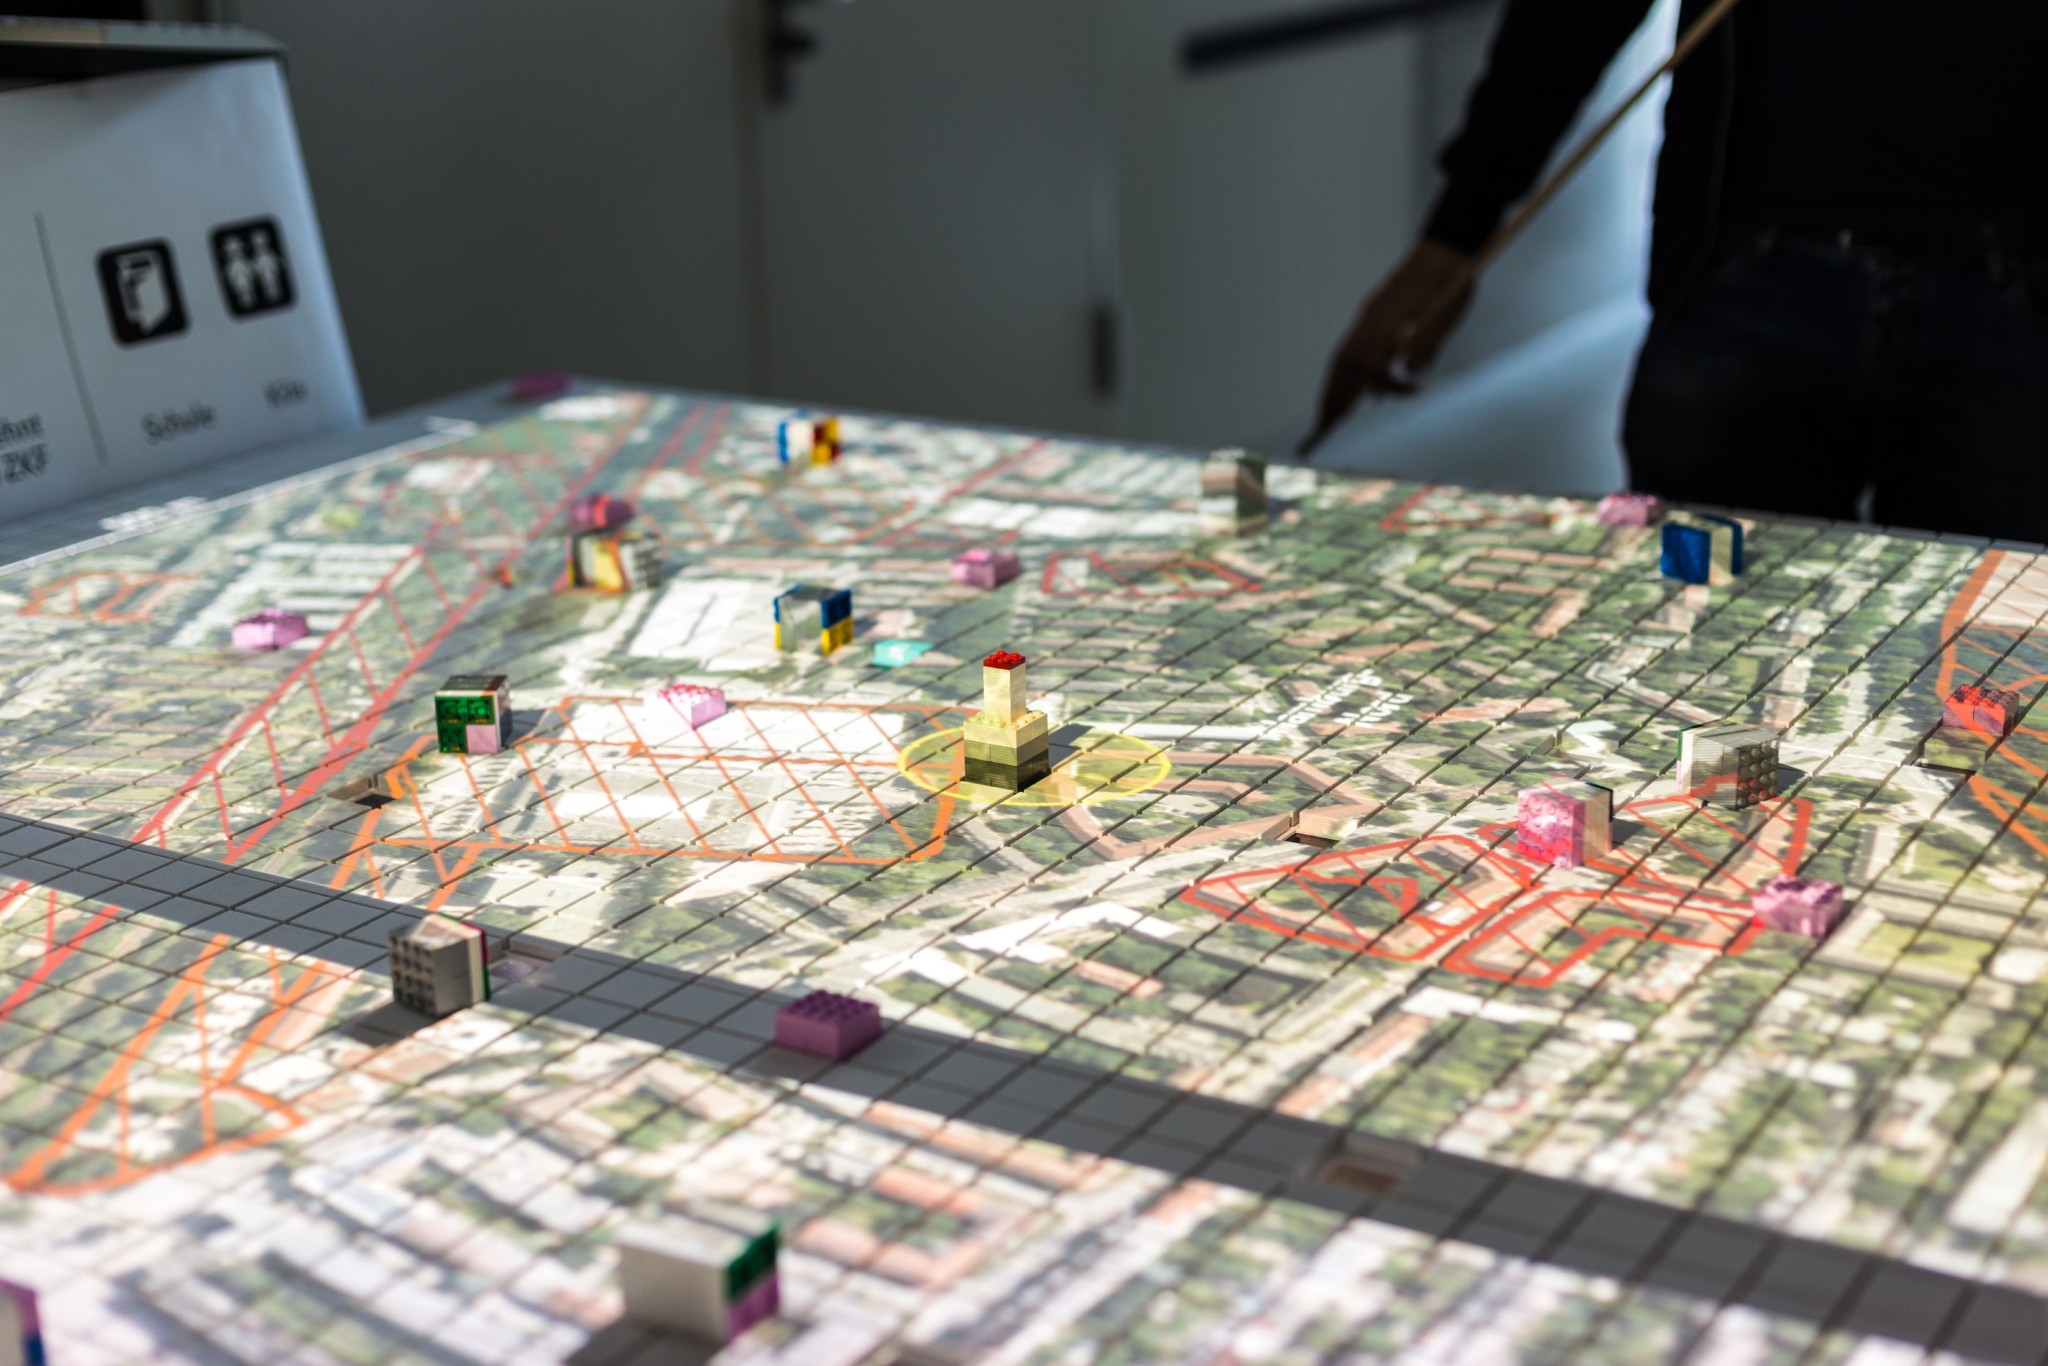
\includegraphics[width=\textwidth]{figures/finidingplaces0.jpg}
  \end{minipage}
    \hfill
   \caption{CityScope FindingPlaces TUI: Users could add or test housing volumes in different configurations. The system would react by prompting on potential risks or issues, such as land contamination, proximity to power-lines, etc.  }
\end{figure}


{The lessons learned about community engagement and public participation using CityScope, were put into extreme test in the \textbf{FindingPlaces} (2015-2016) project. In late '15, the City of Hamburg faced an escalating crisis amidst a massive wave of refugees arriving from war zones in the Middle-East. Here, CityScope FindingPlaces was central in a region-wide effort to construct a public agreement on where and how to host these refugees. CityScope FindingPlaces introduced multiple improvements to current platforms, including agile geographic system, based on real-time GIS, distributed system for interaction instancing, large-scale TUI, as well as a dedicated front-end and back-end architecture. This project also involved an in depth preparation including dedicated participants outreach, orchestrated community sessions, and structured documentation and reporting mechanisms. FindingPlaces proven the ability of CityScope to become pivotal platform for consensus-building amongst diverse stakeholders, that can convert even heated urban debated into tangible solutions.}
\newpage



%%%%%%%%%%%%%%%%%%%%%%%%%%%%%%%%%%%%%%%%%%%%%%%%%%%%%%%%%%%%%%%%%%%%%%%%%%%%%%%%%%%%%%%%%%%%%%%%%%%%%%%%%%%%%%%%%%%%%%%%%%%%%%%%%%%%%%%%%%%%%%%%%%%%%%%%%%%%%%%%%%%%%%%%%%

%%%%%%%%%%%%%%%%%%%%%%%%%%%%%%%%%%%%%%%%%%%%%%%%%%%%%%%%%%%%%%%%%%%%%%%%%%%%%%%%%%%%%%%%%%%%%%%%%%%%%%%%%%%%%%%%%%%%%%%%%%%%%%%%%%%%%%%%%%%%%%%%%%%%%%%%%%%%%%%%%%%%%%%%%%
\section{Proposed Work}

{The bulk of work between this proposal and the dissertation defense would focus on bringing together the four aforementioned themes. Work would consist of three main trajectories: (i) the development of \textbf{CityScopeJS}, a unified CityScope interface for interaction, analysis, and intervention, (ii) further development of \textbf{CityIO}, a backend system for distributed urban analytics modules, and (iii) deployment and integration of CityScope in additional real-world use cases (Hamburg, Vietnam, Andorra, South America, etc).}

\begin{figure}[t]
\begin{center}
    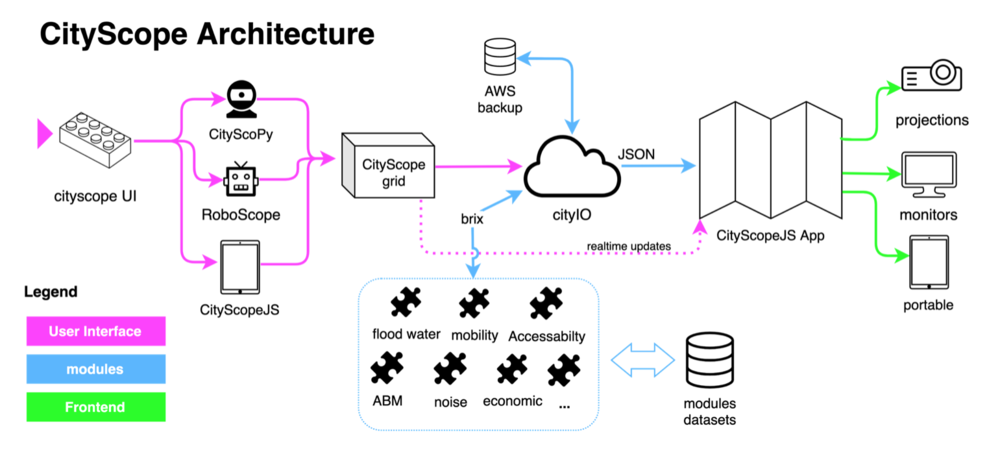
\includegraphics[width=0.8\textwidth]{figures/csjs_arch.png}
\end{center}
   \caption{CityScopeJS and the new CityScope Architecture. This diagram presents the data flow and different components of the current CityScope architecture: (left) different modules control the inputs and grid interaction. (center) upon interaction, cityIO VPC handles the transaction with different urban analytics modules. (right) When these computation phase is complete, the grid and analysis modules results are sent to output devices, either online (CityScopeJS, API), or physical (projectors, monitors)}
\label{fig:csjs_arch}
\end{figure}


{\textbf{CityScopeJS}: A unified interface for the CityScope platform is the \textbf{CityScopeJS} (2018-current) project. This flavor of CityScope attempts to combine many of the aspects of prior tools in one comprehensive and reusable system. In \textbf{CityScope Grasbrook} (2018-2020) and \textbf{CityScope Corktown} (2019-2020) the goal of simulating planning and mobility scenarios was achieved by incorporating interactive, real-time, and collaborative urban planning processes in one web-based, TUI-enabled, modular system.}

\begin{figure}[t]
\begin{center}
    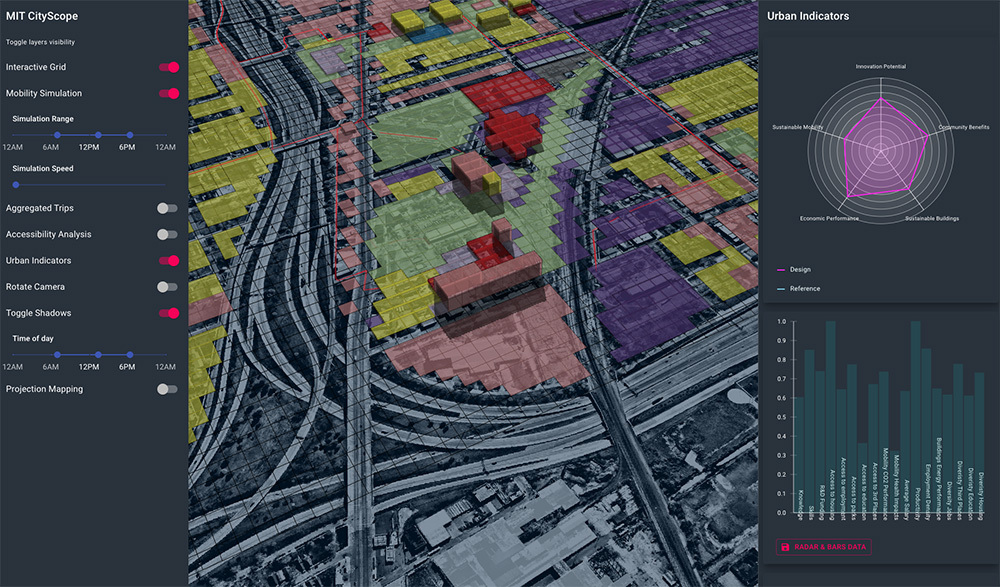
\includegraphics[width=1\textwidth]{figures/csjs.jpg}
\end{center}
   \caption{CityScopeJS interface. As with the TUI versions of CityScope, users interact with a simple, geo-located grid. Interactions are sent to the cityIO analysis modules, and their responses are then displayed spatially as heat-maps, trips, or graphically as charts and data visualisations. The same interface can then be also used with tangible interfaces, robotic UIs, AR or VR.}
\label{fig:csjs}
\end{figure}

{\textbf{CityScope Modules}: At the backend of CityScope, there are growing number of analysis modules design to react in real-time to user interaction. These modules can be global (such as density or shade analysis) or project-site specific (such as accessibility, mobility, storm-water or noise). CityScope is designed to allow both classes of modules to be adapted to most instances of the system. The dissertation will expand on the architecture of the system, its pros and cons, and future prospects.}


{\textbf{Deployments}:The thesis will explore in-progress and future development and implementation of CityScope in Hamburg, Vietnam, Guadalajara, Andorra, as well as other use-cases as they emerge.}


\subsection{Timeline}

\begin{itemize}
\item {2021 - early 2022 -- Finalize new CityScope Architecture development, deployment, and documentation. The goal is to stabilize open-source development efforts of the platform's different components (input - modules/cityIO - UI/output) to allow streamlined deployment for upcoming CS projects.}
	
\item CityScope Corktown: document and submit publication for the CityScope project in Detroit, MI. 

\item {CityScope Grasbrook: complete development and submit publication for the CityScope project in Grasbrook, Hamburg, DE.}
	
\item {Andorra Mobility during COVID-19: Analyze the relationship between COVID-19 spread and the country's mobility pattern retrieved from high-res telecom data. Will complete publication and submit to high-quality venue.}
	
\item {MITOS: Conduct research, development, and deployment of MIT Sustainability Office CityScope project. Investigate impacts of new campus mobility policies in response to COVID-19. Propose feasible interventions via a dynamic CS interface.}  
	
\item {RoboScope: support the development and deploy CityScope robotic interface to the CityScope Volpe platform using CSjs modules.}

\item May 2021 -- Writing. 
\item Feb 2022 -- Defense.
\item April 2022 -- Final changes and submission. 
\end{itemize}
\newpage



%%%%%%%%%%%%%%%%%%%%%%%%%%%%%%%%%%%%%%%%%%%%%%%%%%%%%%%%%%%%%%%%%%%%%%%%%%%%%%%%%%%%%%%%%%%%%%%%%%%%%%%%%%%%%%%%%%%%%%%%%%%%%%%%%%%%%%%%%%%%%%%%%%%%%%%%%%%%%%%%%%%%%%%%%%



